\begin{figure}
    \begin{center}
    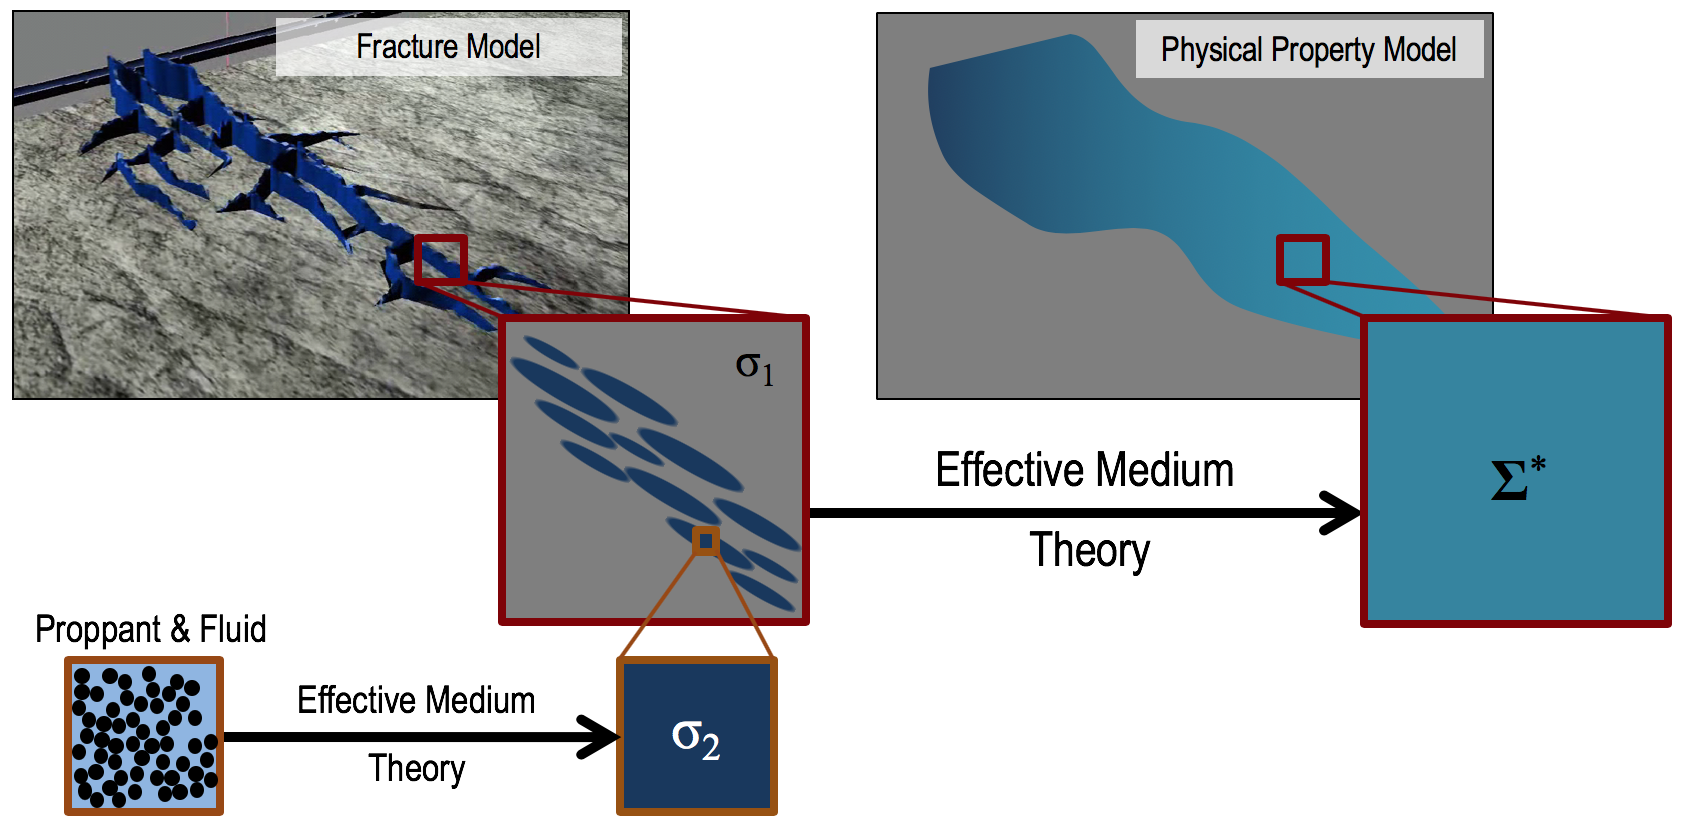
\includegraphics[width=\columnwidth]{figures/phys_prop_model/effective_medium_theory.png}
    \end{center}
\caption{
    Constructing a physical property model for a fractured volume of rock using
    effective medium theory. The electrical conductivity of the proppant fluid
    mixture is given by $\sigma_2$, the conductivity of the background reservoir
    rock by $\sigma_1$. Using effective medium theory, the coarse-scale anisotropic
    conductivity, $\Sigma^*$ describing the fractured volume of rock is computed.
}
\label{fig:effective_medium_theory}
\end{figure}
